% !TEX root = ../main.tex
Saturation occurs when repeated substitutions erase phylogenetic information from an alignment. For two sequences, saturation means that the alignment no longer justifies their inferred evolutionary separation. In larger alignments, the same problem appears at the level of branches. A branch can appear in a maximum-likelihood tree, and can have high conventional support, while the alignment carries little signal for the two groups separated by that branch.

SatuTe generalises saturation between two sequences to a test of saturation between subtrees \cite{manuel2025satute}. A branch \(AB\) splits a site pattern \(\partial\) into subpatterns \(\partial_A\) and \(\partial_B\) on the subtrees \(T_A\) and \(T_B\). The null hypothesis is that the two subtrees evolve independently. Rejection implies phylogenetic signal for branch \(AB\); otherwise, the branch is considered saturated.

The test uses the spectral decomposition of the reversible substitution model \cite{levin2017}. For a site pattern \(\partial\), SatuTe computes partial likelihood vectors \(L(\partial_A)\) and \(L(\partial_B)\). It also computes subtree pattern probabilities \(P(\partial_A)=\langle L(\partial_A),\pi\rangle\) and \(P(\partial_B)=\langle L(\partial_B),\pi\rangle\). With eigenvalues \(\lambda_0=0>\lambda_1\geq\lambda_2\geq\cdots\) and left eigenvectors \(h_i\), the coherence coefficient for a simple eigenvalue is
\begin{equation}
C_{\partial i}
=
\left\langle \frac{L(\partial_A)}{P(\partial_A)}, h_i \right\rangle
\left\langle \frac{L(\partial_B)}{P(\partial_B)}, h_i \right\rangle .
\label{eq-coherence}
\end{equation}
SatuTe uses this coefficient for the second largest eigenvalue. Across \(n\) sites, the empirical statistic is \(\hat C_1=n^{-1}\sum_{s=1}^{n}C_{\partial_s 1}\), with variance estimator \(\hat\sigma_1^2\). The one-sided statistic is \(Z=\sqrt{n}\hat C_1/\hat\sigma_1\). The test rejects subtree independence when \(Z>z_\alpha\).

The second largest eigenvalue gives the slowest non-stationary decay towards the stationary distribution. It is therefore the conservative component on long branches, because all other non-stationary components decay faster. Under general time-reversible nucleotide models \cite{tavare1986} and amino-acid models such as LG, these non-stationary eigenvalues are usually distinct. We ask whether including the faster components changes which branches or alignment regions are called phylogenetically informative when a fitted rate-heterogeneous model separates them.

\begin{figure}[p]
  \vspace*{-2.4cm}
  \centering
  \makebox[\textwidth][c]{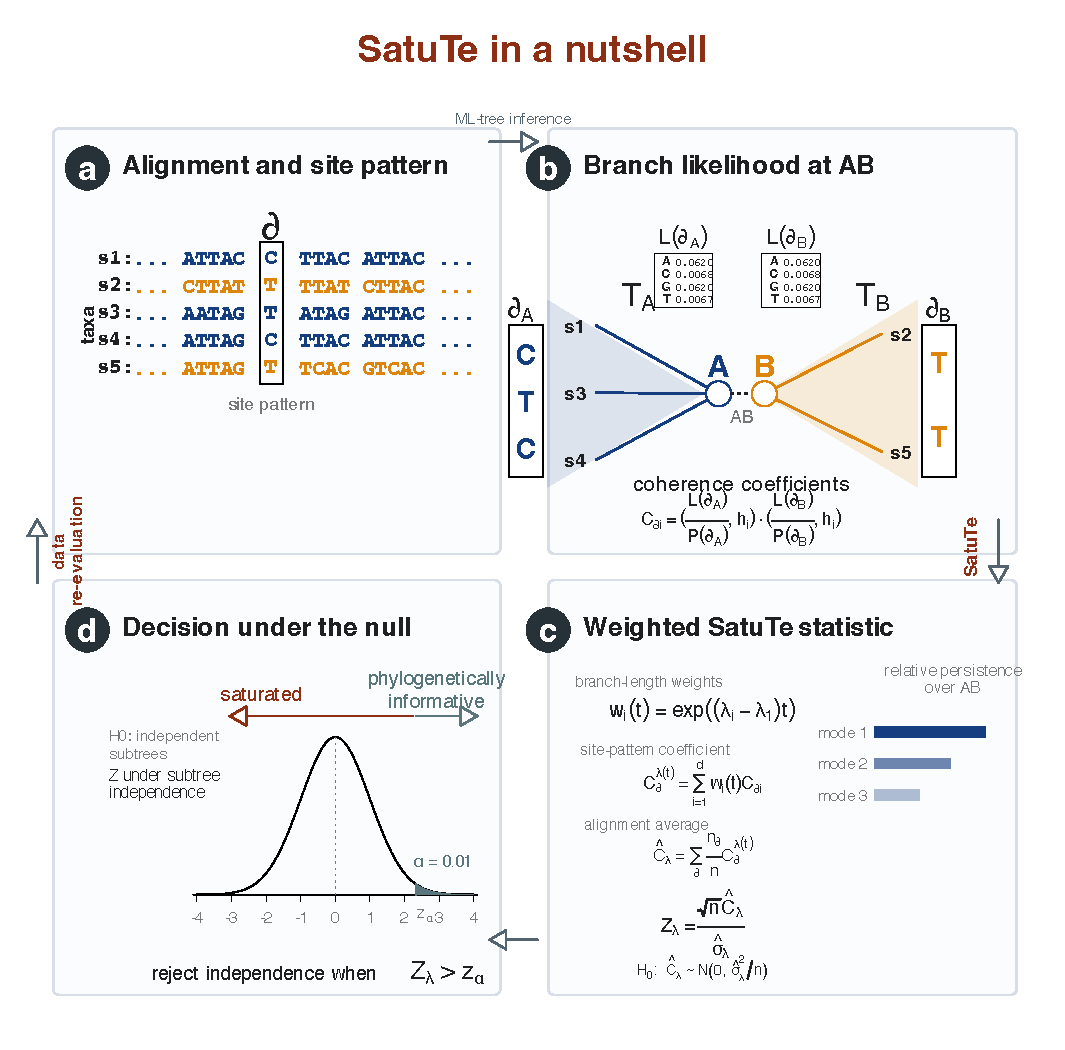
\includegraphics[width=1.10\textwidth]{figures/figure1_satute_weighted_workflow.pdf}}
  \caption{\textbf{SatuTe in a nutshell.} \textbf{a,} Five-taxon DNA alignment where each column represents a pattern \(\partial\). \textbf{b,} The branch \(AB\) splits the five-taxon tree into subtree \(T_A\) with sequences \(S1,S3,S4\) and subtree \(T_B\) with sequences \(S2,S5\). Branch \(AB\) also splits each pattern, such as \(\partial=\text{CTTCT}\), into subpatterns \(\partial_A=\text{CTC}\) and \(\partial_B=\text{TT}\). These subpatterns are used to compute the likelihood vectors \(L(\partial_A)\) and \(L(\partial_B)\), which determine the coherence coefficients. \textbf{c,} The weighted statistic used here keeps the SatuTe coherence coefficients and weights each non-stationary component by its relative persistence over branch length \(t\). \textbf{d,} The null hypothesis of independently evolving subtrees is rejected at the significance level \(\alpha\) if \(Z_\lambda>z_\alpha\). Rejection implies phylogenetic signal for branch \(AB\).}
\end{figure}
